\section{استخراج و کاربرد روابط \lr{Long-channel I-V}}
\label{sec:book-mos-current}
\subsection{فرض‌های مدل و معنای پارامترها}
مدل \lr{Long-channel} را \lr{Ideal}، \lr{First-order} یا \lr{Shockley Model}
نیز می‌نامند. کانال به اندازه‌ای بلند فرض می‌شود که مدل سرعت متناسب با میدان
طولی قابل‌استفاده باشد. \lr{Mobility}، ضخامت مؤثر اکسید و آستانه را در این تحلیل
ثابت می‌گیریم. جریان \lr{Gate} و جریان حالت خاموش صفر فرض می‌شوند. اثرهای
\lr{Velocity Saturation}، \lr{Mobility Degradation} و \lr{Channel Length Modulation}
در بخش \secnum{۲.۴} به تحلیل افزوده می‌شوند \cite[صفحات ۶۴ و ۶۵]{weste}.

در مدل کانال تدریجی، تغییر پتانسیل در امتداد کانال نسبت به تغییر عمودی آن آرام
فرض می‌شود. در نتیجه، بار موضعی را می‌توان با یک رابطه خازنی تقریب زد.
برای محاسبه حاضر، تأثیر تغییر بایاس محلی بر بار \lr{Depletion} در یک آستانه ثابت
خلاصه می‌شود. این فرض‌ها دامنه کاربرد روابط را تعیین می‌کنند.
نمادهای جدول \ref{tab:mos-parameters} پیش از استخراج به کار می‌روند.
\begin{table}[ht]
\centering
\caption{نمادها و واحدهای روابط جریان.}
\label{tab:mos-parameters}
\begin{tabularx}{\textwidth}{rXr}
\toprule
نماد & تعریف & واحد نمونه\\
\midrule
\(W,L\) & عرض کانال و طول مسیر میان \lr{Source} و \lr{Drain} & \unit{\metre}\\
\(t_{\mathrm{ox}}\) & ضخامت اکسید یا ضخامت معادل تعریف‌شده & \unit{\metre}\\
\(\varepsilon_{\mathrm{ox}}\) & \lr{Permittivity} اکسید & \unit{\farad\per\metre}\\
\(C_{\mathrm{ox}}\) & ظرفیت اکسید بر واحد سطح & \unit{\farad\per\metre\squared}\\
\(C_g\) & ظرفیت مدل صفحه‌ای \lr{Gate} و کانال & \unit{\farad}\\
\(\mu_n,\mu_p\) & \lr{Mobility} الکترون و \lr{Hole} & \unit{\metre\squared\per\volt\per\second}\\
\(\beta\) & ضریب فناوری و هندسه در رابطه جریان & \unit{\ampere\per\volt\squared}\\
\(V_{GT}\) & اضافه‌ولتاژ \(V_{GS}-V_{tn}\) در \lr{nMOS} & \unit{\volt}\\
\bottomrule
\end{tabularx}
\end{table}

\subsection{ظرفیت اکسید، هندسه و \lr{EOT}}
طول \(L\) در راستای حرکت حامل از \lr{Source} به \lr{Drain} و عرض \(W\)
در راستای عمود بر آن، روی سطح کانال اندازه‌گیری می‌شود.
در \lr{Strong Inversion}، \lr{Gate} و کانال در دو سوی عایق، تقریباً یک خازن
صفحه‌ای می‌سازند. مساحت مؤثر هندسی \(WL\) است و برای اکسید \lr{SiO\(_2\)} داریم
\begin{equation}
 \varepsilon_{\mathrm{ox}}=3.9\varepsilon_0,\qquad
 C_{\mathrm{ox}}=\frac{\varepsilon_{\mathrm{ox}}}{t_{\mathrm{ox}}},\qquad
 C_g=C_{\mathrm{ox}}WL.
 \label{eq:mos-oxide-cap}
\end{equation}
\(\varepsilon_0\approx\qty{8.85e-12}{\farad\per\metre}\) است.
در واحد سانتی‌متری کتاب، همین مقدار
\qty{8.85e-14}{\farad\per\centi\metre} نوشته می‌شود
\cite[رابطه \secnum{۲.۲}، شکل \secnum{۲.۶}]{weste}.
با نصف‌شدن ضخامت، ظرفیت بر واحد سطح دو برابر می‌شود. با دوبرابرشدن عرض، ظرفیت
کل دو برابر می‌شود. \(C_{\mathrm{ox}}\) و \(C_g\) واحد و نقش متفاوتی دارند.

برای نمونه فرضی \(t_{\mathrm{ox}}=\qty{10}{\nano\metre}\)،
\(W=\qty{1}{\micro\metre}\) و \(L=\qty{0.5}{\micro\metre}\)، ابتدا همه طول‌ها
را به متر می‌بریم. چون \(\qty{10}{\nano\metre}=10^{-8}\,\unit{\metre}\)، داریم
\begin{align*}
 C_{\mathrm{ox}}&=\frac{3.9(8.85\times10^{-12})}{10^{-8}}
 =3.4515\times10^{-3}\,\unit{\farad\per\metre\squared},\\
 C_g&=(3.4515\times10^{-3})(10^{-6})(0.5\times10^{-6})\,\unit{\farad}
 \approx\qty{1.73}{\femto\farad}.
\end{align*}
ضریب تبدیل مساحت از \unit{\micro\metre\squared} به \unit{\metre\squared}
برابر \(10^{-12}\) است، زیرا هر دو بعد در \(10^{-6}\) ضرب می‌شوند.
این ظرفیت صفحه‌ای، پایه استخراج جریان است. تقسیم آن میان پایانه‌ها در بخش
\secnum{۲.۳} بررسی می‌شود.

برای عایق \lr{High-k}، \lr{Equivalent Oxide Thickness} یا \lr{EOT} را ضخامت
لایه فرضی \lr{SiO\(_2\)} با همان \(C_{\mathrm{ox}}\) تعریف می‌کنند
\cite[صفحه ۶۶]{weste}. اگر ضخامت فیزیکی عایق \(t_h\) و گذردهی آن
\(\varepsilon_h\) باشد، از برابرگرفتن ظرفیت بر واحد سطح نتیجه می‌شود
\begin{equation}
 \frac{\varepsilon_h}{t_h}=\frac{\varepsilon_{\mathrm{ox}}}{\mathrm{EOT}}
 \quad\Longrightarrow\quad
 \mathrm{EOT}=t_h\frac{\varepsilon_{\mathrm{ox}}}{\varepsilon_h}.
 \label{eq:mos-eot}
\end{equation}
اگر گذردهی چهار برابر و ضخامت فیزیکی \qty{4}{\nano\metre} باشد،
\(\mathrm{EOT}=\qty{1}{\nano\metre}\) می‌شود. در این مثال، ضخامت فیزیکی بیشتر
با ظرفیت معادل همان اکسید نازک سازگار است.

\subsection{بار کانال در توضیح متوسط کتاب}
بار روی خازن به ولتاژ دو سوی همان خازن وابسته است. پتانسیل کانال میان
\(V_S\) و \(V_D\) تغییر می‌کند. کتاب برای استخراج مقدماتی، پتانسیل نماینده کانال
را میانگین دو انتها می‌گیرد و می‌نویسد
\begin{align}
 V_c&\approx\frac{V_S+V_D}{2}=V_S+\frac{V_{DS}}2,\notag\\
 V_{gc}&\approx V_G-V_c=V_{GS}-\frac{V_{DS}}2.
 \label{eq:mos-mean-potential}
\end{align}
برای تشکیل بار متحرک، ولتاژ باید از آستانه عبور کند. با تعریف بزرگی بار کانال
\(Q_{\mathrm{ch}}\ge0\)، رابطه مقدماتی کتاب چنین بازنویسی می‌شود
\begin{equation}
 Q_{\mathrm{ch}}\approx C_g(V_{gc}-V_{tn})
 \approx C_{\mathrm{ox}}WL\left(V_{GT}-\frac{V_{DS}}2\right).
 \label{eq:mos-average-charge}
\end{equation}
این توضیح از رابطه \secnum{۲.۱} کتاب و اسلاید ۱۵ گرفته شده است.
علامت بار الکترون‌ها منفی است. در این رابطه با بزرگی آن کار می‌کنیم.
افزایش \(V_{GS}\) بار متحرک را بیشتر می‌کند. افزایش \(V_{DS}\) با ثابت‌ماندن
\(V_{GS}\)، اضافه‌ولتاژ مؤثر نزدیک \lr{Drain} را کم می‌کند.

میانگین دو ولتاژ انتهایی یک ساده‌سازی برای استخراج مقدماتی است.
پتانسیل واقعی در طول کانال الزاماً خطی با مکان تغییر نمی‌کند، بنابراین
\eqref{eq:mos-average-charge} را به عنوان تقریب بزرگی کل بار به کار می‌بریم.
استخراج با بار موضعی در ادامه، همان رابطه جریان را در مدل کانال تدریجی به دست می‌دهد
و نیاز به فرض خطی‌بودن پتانسیل مکانی را برمی‌دارد.

\subsection{\lr{Mobility}، میدان طولی و زمان عبور}
\lr{Mobility} ضریب تبدیل بزرگی میدان الکتریکی به سرعت متوسط رانش در مدل میدان
کم است. اگر \(v\) بزرگی سرعت و \(E\) بزرگی میدان طولی باشد، داریم
\begin{equation}
 v=\mu_n E,\qquad E\approx\frac{V_{DS}}L,\qquad
 t_{\mathrm{tr}}\approx\frac Lv.
 \label{eq:mos-drift}
\end{equation}
رابطه‌های \secnum{۲.۳} و \secnum{۲.۴} کتاب و اسلاید ۱۶ همین مسیر را بیان می‌کنند.
\(t_{\mathrm{tr}}\) زمان عبور حامل در این تصویر مقدماتی است. تأخیر گیت به جریان
شارژ و تخلیه بار خارجی نیز وابسته است.

برای فهم واحد \(\mu\)، میدان واحد \unit{\volt\per\metre} دارد و سرعت واحد
\unit{\metre\per\second}. پس واحد ضریب تناسب
\unit{\metre\squared\per\volt\per\second} است. تبدیل واحد رایج کتاب چنین است
\begin{equation*}
 \qty{1}{\centi\metre\squared\per\volt\per\second}
 =10^{-4}\,\unit{\metre\squared\per\volt\per\second}.
\end{equation*}
کتاب برای الکترون در میدان کم حدود \num{500} تا
\qty{700}{\centi\metre\squared\per\volt\per\second}
را ذکر می‌کند و سپس کاهش \lr{Mobility} در میدان‌های قوی را یادآور می‌شود
\cite[صفحه ۶۶]{weste}. مقدار مناسب هر مثال باید از داده همان مثال برداشته شود.

در مثال فرضی \(L=\qty{1}{\micro\metre}\)، \(V_{DS}=\qty{0.1}{\volt}\)
و \(\mu_n=\qty{500}{\centi\metre\squared\per\volt\per\second}\)، داریم
\[
 E\approx\frac{0.1}{10^{-6}}=10^5\,\unit{\volt\per\metre},\qquad
 v\approx(0.05)(10^5)=\qty{5000}{\metre\per\second},\qquad
 t_{\mathrm{tr}}\approx\qty{0.2}{\nano\second}.
\]
در این محاسبه، تناسب سرعت با میدان و تقریب میدان متوسط فرض شده‌اند.

\subsection{استخراج رابطه \lr{Linear} با روش کتاب}
جریان، بار عبوری در واحد زمان است. در تصویر بار متوسط و زمان عبور متوسط،
جریان برابر \(Q_{\mathrm{ch}}/t_{\mathrm{tr}}\) تخمین زده می‌شود.
با جای‌گذاری \eqref{eq:mos-average-charge} و \eqref{eq:mos-drift}، مراحل حذف
عامل‌ها را به صورت زیر دنبال می‌کنیم
\begin{align}
 I_{DS}&\approx\frac{Q_{\mathrm{ch}}}{L/v}
 =Q_{\mathrm{ch}}\frac vL,\notag\\
 &\approx C_{\mathrm{ox}}WL\left(V_{GT}-\frac{V_{DS}}2\right)
 \frac{\mu_n V_{DS}}{L^2},\notag\\
 &=\mu_n C_{\mathrm{ox}}\frac WL
 \left(V_{GT}V_{DS}-\frac{V_{DS}^2}{2}\right).
 \label{eq:mos-book-linear}
\end{align}
از یک عامل \(L\) در صورت و دو عامل \(L\) در مخرج، نسبت \(1/L\) باقی می‌ماند.
با معرفی پارامتر فناوری \(k'_n\) و پارامتر فناوری و هندسه \(\beta_n\)، داریم
\begin{equation}
 k'_n=\mu_n C_{\mathrm{ox}},\qquad
 \beta_n=k'_n\frac WL=\mu_n C_{\mathrm{ox}}\frac WL.
 \label{eq:mos-beta}
\end{equation}
پس رابطه مدل برای \(V_{GS}>V_{tn}\) و \(0\le V_{DS}\le V_{GT}\) چنین است
\begin{equation}
 \boxed{I_{DS}=\beta_n\left[(V_{GS}-V_{tn})V_{DS}-\frac{V_{DS}^2}{2}\right].}
 \label{eq:mos-linear}
\end{equation}
این رابطه با روابط \secnum{۲.۵} تا \secnum{۲.۷} کتاب و اسلاید ۱۷ سازگار است.
علامت مساوی در \eqref{eq:mos-linear} بیانگر رابطه تعریف‌شده در مدل ایدئال است.

واحد \(\mu C_{\mathrm{ox}}\) برابر
\(\unit{\farad\per\volt\per\second}=\unit{\ampere\per\volt\squared}\) است.
نسبت \(W/L\) بی‌بعد است. داخل کروشه دو جمله با واحد \unit{\volt\squared}
داریم و حاصل، جریان با واحد \unit{\ampere} است.
برخی منابع، عامل \(1/2\) را در تعریف \(k'\) یا ضریب جریان جذب می‌کنند.
پانوشت صفحه ۶۶ کتاب نیز این تفاوت را یادآوری می‌کند.
پیش از استفاده از مقدار نقل‌شده، تعریف ضریب را با \eqref{eq:mos-beta} مقایسه می‌کنیم.

\subsection{استخراج تکمیلی با بار موضعی و انتگرال}
برای دقیق‌ترکردن استدلال در چارچوب همان مدل، مکان \(x\) را از \lr{Source}
در \(x=0\) تا \lr{Drain} در \(x=L\) تعریف می‌کنیم. \(V(x)\) پتانسیل محلی
نسبت به \lr{Source} است. پس \(V(0)=0\) و \(V(L)=V_{DS}\).
در قطعه کوچکی به طول \(dx\)، بزرگی بار متحرک کانال برابر است با
\begin{equation}
 dQ_{\mathrm{ch}}=W C_{\mathrm{ox}}[V_{GT}-V(x)]\,dx.
 \label{eq:mos-local-charge}
\end{equation}
عبارت \(C_{\mathrm{ox}}[V_{GT}-V(x)]\) بار بر واحد سطح و
\(Wdx\) سطح قطعه است. بار علامت‌دار الکترون‌ها، منفی این مقدار است.

زمان عبور از همین قطعه \(dt=dx/v(x)\) و بزرگی سرعت رانش
\(v(x)=\mu_n\,dV/dx\) است. این رابطه از بزرگی میدان استفاده می‌کند.
با تقسیم بار عبوری بر زمان و فرض جریان پایدار در طول کانال، داریم
\begin{equation}
 I_{DS}=W\mu_nC_{\mathrm{ox}}[V_{GT}-V(x)]\frac{dV}{dx}.
 \label{eq:mos-local-current}
\end{equation}
در جریان پایدار، بار در هیچ قطعه‌ای انباشته نمی‌شود، بنابراین جریان عبوری از
همه مقطع‌ها یکسان است. دو طرف را در \(dx\) ضرب و در طول کانال جمع می‌کنیم.
نماد انتگرال، جمع پیوسته سهم قطعه‌های کوچک است. با تغییر متغیر از مکان به
پتانسیل، جمع از صفر تا \(V_{DS}\) انجام می‌شود
\begin{equation*}
 \int_0^L I_{DS}\,dx
 =W\mu_nC_{\mathrm{ox}}\int_0^{V_{DS}}(V_{GT}-V)\,dV.
\end{equation*}
سمت چپ چون جریان ثابت است، \(I_{DS}L\) می‌شود. در سمت راست، مساحت زیر خط
\(V_{GT}-V\) در بازه صفر تا \(V_{DS}\)، مساحت یک مستطیل به ارتفاع \(V_{GT}\)
منهای مساحت مثلث به ارتفاع و قاعده \(V_{DS}\) است. پس
\begin{equation*}
 I_{DS}L=W\mu_n C_{\mathrm{ox}}
 \left(V_{GT}V_{DS}-\frac12V_{DS}^2\right).
\end{equation*}
تقسیم بر \(L\)، دقیقاً رابطه \eqref{eq:mos-linear} را در فرض‌های مدل به دست
می‌دهد. عامل یک‌دوم از تغییر بار در امتداد کانال ناشی می‌شود. شرط
\(V_{DS}\le V_{GT}\) تضمین می‌کند بار موضعی در سراسر کانال نامنفی باقی بماند.

\subsection{تقریب مقاومتی و مرز \lr{Saturation}}
برای \(V_{DS}\ll V_{GT}\)، جمله مربعی نسبت به جمله اول کوچک است. نسبت بزرگی
آن دو جمله \(V_{DS}/(2V_{GT})\) است. با حذف جمله کوچک، داریم
\begin{equation}
 I_{DS}\approx\beta_nV_{GT}V_{DS},\qquad
 R_{\mathrm{on}}\approx\frac{V_{DS}}{I_{DS}}
 \approx\frac1{\beta_nV_{GT}}.
 \label{eq:mos-small-vds}
\end{equation}
مقاومت تقریبی با ولتاژ \lr{Gate} کنترل می‌شود.
در رابطه کامل ناحیه \lr{Linear}، نسبت \(V_{DS}/I_{DS}\) برابر
\(1/[\beta_n(V_{GT}-V_{DS}/2)]\) است و با ولتاژ تغییر می‌کند.

برای \(\beta_n=\qty{200}{\micro\ampere\per\volt\squared}\)،
\(V_{GT}=\qty{0.8}{\volt}\) و \(V_{DS}=\qty{0.1}{\volt}\)، جریان کامل
به صورت زیر محاسبه می‌شود.
\[
 200[0.8(0.1)-0.1^2/2]=\qty{15}{\micro\ampere}.
\]
تقریب مقاومتی \qty{16}{\micro\ampere} می‌دهد، حدود \num{6.7} درصد بیشتر از مقدار
رابطه کامل. برای کاهش خطای این تقریب باید نسبت \(V_{DS}/V_{GT}\) کوچک‌تر شود.

در مرز تشکیل \lr{Pinch-off}، \(V_{GD}=V_{tn}\)، بنابراین ولتاژ اشباع در مدل
بلندکانال برابر است با
\begin{equation}
 V_{DS,\mathrm{sat}}=V_{GT}=V_{GS}-V_{tn}.
 \label{eq:mos-vdsat}
\end{equation}
با جای‌گذاری همین مقدار در \eqref{eq:mos-linear}، داریم
\begin{align}
 I_{DS,\mathrm{sat}}
 &=\beta_n\left(V_{GT}^2-\frac{V_{GT}^2}{2}\right)
 =\frac{\beta_n}{2}V_{GT}^2,\notag\\
 &\boxed{I_{DS,\mathrm{sat}}=\frac{\beta_n}{2}(V_{GS}-V_{tn})^2.}
 \label{eq:mos-saturation}
\end{align}
این رابطه برای \(V_{GS}>V_{tn}\) و \(V_{DS}\ge V_{DS,\mathrm{sat}}\) به کار
می‌رود \cite[رابطه \secnum{۲.۸} و اسلاید ۱۸]{weste,mos}.
پس از مرز، افزایش ولتاژ \lr{Drain} عمدتاً روی ناحیه نزدیک \lr{Drain} می‌افتد.
در تقریبِ طول مؤثر ثابت، جریان به مقدار مرزی محدود می‌شود.

می‌توان رابطه \lr{Linear} را با کامل‌کردن مربع نیز بازنوشت
\begin{equation}
 I_{DS}=\frac{\beta_n}{2}
 \left[V_{GT}^2-(V_{GT}-V_{DS})^2\right],\qquad 0\le V_{DS}\le V_{GT}.
 \label{eq:mos-complete-square}
\end{equation}
در مرز، مربع دوم صفر و جریان برابر بیشینه این قطعه است.
برای \(V_{DS}>V_{GT}\)، فرض بار نامنفی تا انتهای کانال از اعتبار می‌افتد و
قطعه اشباع انتخاب می‌شود. همین انتخاب از افت مصنوعی جریان ناشی از ادامه‌دادن
سهمی به بیرون بازه جلوگیری می‌کند.

\subsection{رابطه قطعه‌ای، پیوستگی و جریان‌های \lr{Ion} و \lr{Ioff}}
برای \(V_{DS}\ge0\)، مدل جریان را با شرط‌ها یکجا می‌نویسیم
\begin{equation}
 I_{DS}=\begin{cases}
 0,&V_{GS}\le V_{tn},\\[2pt]
 \beta_n(V_{GT}V_{DS}-V_{DS}^2/2),
 &V_{GS}>V_{tn},\quad 0\le V_{DS}<V_{GT},\\[2pt]
 \beta_n V_{GT}^2/2,
 &V_{GS}>V_{tn},\quad V_{DS}\ge V_{GT}.
 \end{cases}
 \label{eq:mos-piecewise}
\end{equation}
این صورت، مرزهای رابطه \secnum{۲.۱۰} کتاب و اسلاید ۱۹ را نیز پوشش می‌دهد.
در \(V_{DS}=0\)، قطعه \lr{Linear} جریان صفر می‌دهد. در
\(V_{DS}=V_{GT}\)، دو قطعه مقدار \(\beta_n V_{GT}^2/2\) می‌دهند.
با \(V_{GS}\) نزدیک آستانه از بالا، جریان اشباع به صفر میل می‌کند.
در هر سه بررسی، رفتار قطعه‌ای پیوسته است.

کتاب \(I_{\mathrm{on}}\) را جریان در \(V_{GS}=V_{DS}=V_{DD}\)، و
\(I_{\mathrm{off}}\) را جریان در \(V_{GS}=0,V_{DS}=V_{DD}\) تعریف می‌کند.
برای \(V_{DD}>V_{tn}>0\)، شرط اشباع برای حالت روشن برقرار است و داریم
\begin{equation}
 I_{\mathrm{on}}=\frac{\beta_n}{2}(V_{DD}-V_{tn})^2,\qquad
 I_{\mathrm{off}}=0\quad\text{\rl{در مدل مرتبه اول}}.
 \label{eq:mos-ion-ioff}
\end{equation}
اگر \(V_{DD}\le V_{tn}\) باشد، همین مدل جریان حالت روشن را نیز صفر می‌گیرد.
این شرط پیش از مربع‌کردن اختلاف بررسی می‌شود. جریان خاموش واقعی در درس
\lr{Leakage} تحلیل خواهد شد \cite[رابطه \secnum{۲.۹}]{weste}.

در \lr{Saturation}، دوبرابرشدن \(W\) با بقیه پارامترهای ثابت، جریان را دو برابر
می‌کند. دوبرابرشدن \(L\) جریان را نصف می‌کند، مشروط به حفظ اعتبار مدل و پارامترها.
دوبرابرشدن \(V_{GT}\) جریان را چهار برابر می‌کند. برای تغییر \(V_{GS}\)،
ابتدا آستانه را کم می‌کنیم و سپس توان دو می‌گیریم.
\clearpage

\subsection{حل مثال اسلاید ۲۰ با واحدهای سازگار}
داده‌های اسلاید ۲۰ عبارت‌اند از \(t_{\mathrm{ox}}=\qty{10}{\nano\metre}\)،
\(\mu_n=\qty{350}{\centi\metre\squared\per\volt\per\second}\)،
\(V_{tn}=\qty{0.7}{\volt}\) و \(W/L=4/2=2\) \cite{mos}.
در اسلاید، ضخامت به صورت \(100\) \lr{angstrom} داده شده است.
هر \lr{angstrom} برابر \(10^{-10}\,\unit{\metre}\) است، پس
\(100\) \lr{angstrom} برابر \qty{10}{\nano\metre} می‌شود.

با واحد متر، \(\mu_n=0.035\,\unit{\metre\squared\per\volt\per\second}\)
و \(C_{\mathrm{ox}}=3.4515\times10^{-3}\,\unit{\farad\per\metre\squared}\) است.
بنابراین
\begin{align*}
 k'_n&=(0.035)(3.4515\times10^{-3})\,
 \unit{\ampere\per\volt\squared}
 \approx\qty{120.8}{\micro\ampere\per\volt\squared},\\
 \beta_n&=k'_n\frac WL\approx\qty{241.6}{\micro\ampere\per\volt\squared}.
\end{align*}
اسلاید ضریب \(k'_n\) را حدود \qty{120}{\micro\ampere\per\volt\squared}
گزارش می‌کند. برای هماهنگی با دقت همان مثال، در ادامه
\(\beta_n=\qty{240}{\micro\ampere\per\volt\squared}\) می‌گیریم.
وقتی \(V_{GS}=\qty{3}{\volt}\)، اضافه‌ولتاژ \(V_{GT}=\qty{2.3}{\volt}\) است.
برای \(V_{DS}=\qty{1}{\volt}\)، ناحیه \lr{Linear} و جریان
\[
 I_{DS}=240\left[2.3(1)-\frac{1^2}{2}\right]\,\unit{\micro\ampere}
 =\qty{432}{\micro\ampere}
\]
می‌شود. برای \(V_{DS}=\qty{4}{\volt}\)، ناحیه \lr{Saturation} و جریان
\[
 I_{DS}=\frac{240}{2}(2.3)^2\,\unit{\micro\ampere}
 =\qty{634.8}{\micro\ampere}\approx\qty{0.635}{\milli\ampere}
\]
است. مقدار \(V_{DS}=\qty{2.3}{\volt}\) در هر دو فرمول همین پاسخ را می‌دهد.
منحنی‌های شکل \ref{fig:mos-slide-curves} با همین ضریب گرد‌شده محاسبه شده‌اند.

\begin{figure}[ht]
\centering
\begin{latin}
\PersianMathDigits
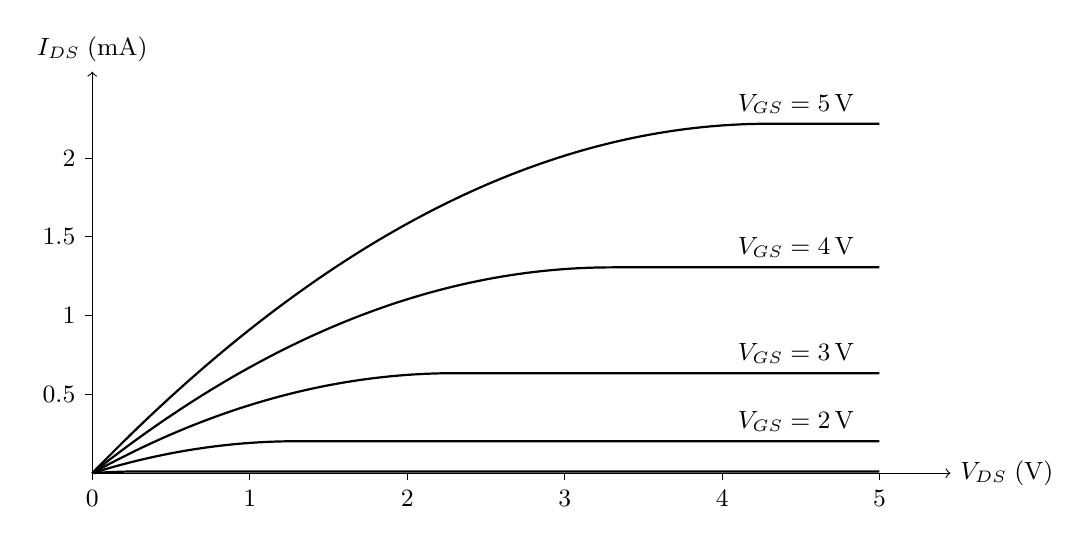
\begin{tikzpicture}[x=2cm,y=2cm,font=\small]
\draw[->] (0,0)--(5.45,0) node[right] {$V_{DS}\;(\mathrm V)$};
\draw[->] (0,0)--(0,2.55) node[above] {$I_{DS}\;(\mathrm{mA})$};
\foreach \x in {0,1,2,3,4,5}{\draw (\x,0)--(\x,-0.045) node[below] {$\x$};}
\foreach \y in {0.5,1,1.5,2}{\draw (0,\y)--(-0.045,\y) node[left] {$\y$};}
\foreach \g in {1,2,3,4,5}{
 \draw[thick,domain=0:5,samples=101] plot (\x,{0.24*((\g-0.7)*min(\x,\g-0.7)-0.5*min(\x,\g-0.7)^2)});
}
\node[anchor=south east] at (4.9,2.22) {$V_{GS}=5\,\mathrm V$};
\node[anchor=south east] at (4.9,1.307) {$V_{GS}=4\,\mathrm V$};
\node[anchor=south east] at (4.9,0.635) {$V_{GS}=3\,\mathrm V$};
\node[anchor=south east] at (4.9,0.203) {$V_{GS}=2\,\mathrm V$};
\end{tikzpicture}
\end{latin}
\caption{مشخصه‌های محاسبه‌شده از مدل \lr{Long-channel} با داده اسلاید ۲۰ و
\(\beta_n=\qty{240}{\micro\ampere\per\volt\squared}\). منحنی \(V_{GS}=0\)
روی محور افقی است و پایین‌ترین منحنی غیرصفر به \(V_{GS}=\qty{1}{\volt}\) مربوط است.
نمودار، بازتولید مدل ایدئال با فرض‌های بیان‌شده است \cite{mos}.}
\label{fig:mos-slide-curves}
\end{figure}

\subsection{حل مثال \texorpdfstring{\secnum{۲.۱}}{۲.۱} کتاب و اختلاف عدد ضریب}
در مثال \secnum{۲.۱} کتاب، نام فناوری \qty{65}{\nano\metre} است، اما طول رسم‌شده
\(L=\qty{50}{\nano\metre}\) و \(W=\qty{100}{\nano\metre}\) داده شده است.
برای محاسبه \(W/L\)، ابعاد واقعی داده‌شده را به کار می‌بریم. سایر داده‌ها
\(t_{\mathrm{ox}}=\qty{1.05}{\nano\metre}\)،
\(\mu_n=\qty{80}{\centi\metre\squared\per\volt\per\second}\) و
\(V_{tn}=\qty{0.3}{\volt}\) در دمای ذکرشده \qty{70}{\degreeCelsius} هستند
\cite[صفحه ۶۷]{weste}.

تبدیل‌ها \(\mu_n=0.008\,\unit{\metre\squared\per\volt\per\second}\)،
\(t_{\mathrm{ox}}=1.05\times10^{-9}\,\unit{\metre}\) و \(W/L=2\) می‌دهند.
پس با ثابت \(\varepsilon_0\) درج‌شده در کتاب داریم
\begin{align}
 C_{\mathrm{ox}}&=\frac{3.9(8.85\times10^{-12})}{1.05\times10^{-9}}
 \approx0.03287\,\unit{\farad\per\metre\squared},\notag\\
 k'_n&\approx(0.008)(0.03287)
 \approx\qty{263}{\micro\ampere\per\volt\squared},\notag\\
 \beta_n&\approx\qty{526}{\micro\ampere\per\volt\squared}.
 \label{eq:mos-book-beta}
\end{align}
در رابطه \secnum{۲.۱۱} چاپ کتاب، ضریب پیش از \(W/L\) برابر
\qty{262}{\micro\ampere\per\volt\squared} نوشته شده است.
محاسبه از داده‌های درج‌شده حدود \qty{263}{\micro\ampere\per\volt\squared}
می‌دهد. اختلاف حدود \num{0.4} درصد است. برای سازگاری داخلی، جدول و نمودار این جزوه
همگی با \(\beta_n=\qty{526}{\micro\ampere\per\volt\squared}\) محاسبه شده‌اند.

برای \(V_{GS}=0\) و \qty{0.2}{\volt}، شرط روشن‌شدن برقرار نیست.
برای چهار مقدار بعدی، جدول \ref{tab:mos-book-points} ولتاژ مرزی و جریان اشباع
را نشان می‌دهد. مثلاً در \(V_{GS}=\qty{0.8}{\volt}\)،
\(V_{GT}=\qty{0.5}{\volt}\) و جریان اشباع
\((526/2)(0.5)^2=\qty{65.75}{\micro\ampere}\) است.
\begin{table}[ht]
\centering
\caption{نقاط مرزی مثال کتاب، با ضریب محاسبه‌شده و گرد‌شده در \eqref{eq:mos-book-beta}.}
\label{tab:mos-book-points}
\begin{tabular}{ccc}
\toprule
\(V_{GS}\;(\unit{\volt})\)&\(V_{DS,\mathrm{sat}}\;(\unit{\volt})\)&
\(I_{DS,\mathrm{sat}}\;(\unit{\micro\ampere})\)\\
\midrule
\(0.4\)&\(0.1\)&\(2.63\)\\
\(0.6\)&\(0.3\)&\(23.67\)\\
\(0.8\)&\(0.5\)&\(65.75\)\\
\(1.0\)&\(0.7\)&\(128.87\)\\
\bottomrule
\end{tabular}
\end{table}

برای رسم هر منحنی، از صفر تا \(V_{DS,\mathrm{sat}}\) رابطه \lr{Linear} و پس از
آن رابطه \lr{Saturation} به کار می‌رود. شکل \ref{fig:mos-book-curves} نتیجه را
نمایش می‌دهد. افزاره کوچک این مثال، از نظر فیزیکی اثرهای میدان قوی دارد.
کتاب صریحاً استفاده از مدل ایدئال را برای این تمرین خواسته و اثرهای اصلاحی را
به بخش بعد ارجاع داده است.
\begin{figure}[ht]
\centering
\begin{latin}
\PersianMathDigits
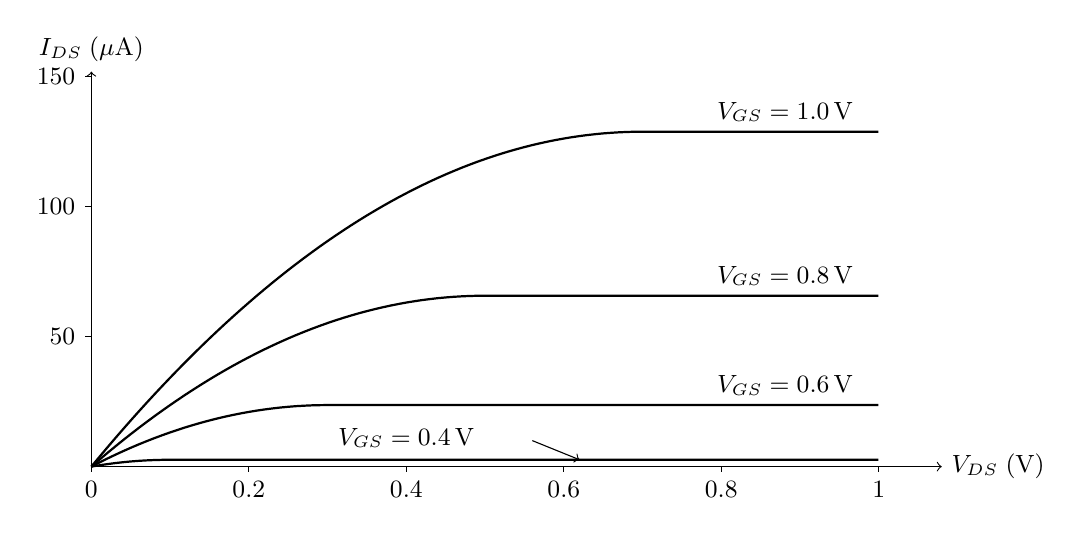
\begin{tikzpicture}[x=10cm,y=0.033cm,font=\small]
\draw[->] (0,0)--(1.08,0) node[right] {$V_{DS}\;(\mathrm V)$};
\draw[->] (0,0)--(0,152) node[above] {$I_{DS}\;(\mathrm{\mu A})$};
\foreach \x in {0,0.2,0.4,0.6,0.8,1}{\draw (\x,0)--(\x,-2) node[below] {$\x$};}
\foreach \y in {50,100,150}{\draw (0,\y)--(-0.008,\y) node[left] {$\y$};}
\foreach \g in {0.4,0.6,0.8,1.0}{
 \draw[thick,domain=0:1,samples=101] plot (\x,{526*((\g-0.3)*min(\x,\g-0.3)-0.5*min(\x,\g-0.3)^2)});
}
\node[anchor=south east] at (0.98,128.87) {$V_{GS}=1.0\,\mathrm V$};
\node[anchor=south east] at (0.98,65.75) {$V_{GS}=0.8\,\mathrm V$};
\node[anchor=south east] at (0.98,23.67) {$V_{GS}=0.6\,\mathrm V$};
\draw[->] (0.56,10)--(0.62,2.63);
\node at (0.40,11) {$V_{GS}=0.4\,\mathrm V$};
\end{tikzpicture}
\end{latin}
\caption{منحنی‌های مدل ایدئال مثال \secnum{۲.۱} کتاب با
\(\beta_n=\qty{526}{\micro\ampere\per\volt\squared}\).
دو منحنی \(V_{GS}=0\) و \(V_{GS}=\qty{0.2}{\volt}\) روی محور افقی قرار دارند
\cite[شکل \secnum{۲.۷}]{weste}.}
\label{fig:mos-book-curves}
\end{figure}

\subsection{\lr{pMOS} با بزرگی مثبت و سپس قرارداد علامت‌دار}
برای \lr{pMOS}، \lr{Source} پایانه پرپتانسیل‌تر است. آستانه علامت‌دار را
\(V_{tp}<0\) و بزرگی مثبت آن را \(V_{TP}=|V_{tp}|\) می‌نامیم.
ولتاژها و ضریب مثبت را به صورت زیر تعریف می‌کنیم
\begin{equation}
 V_{SG}=V_S-V_G,\quad V_{SD}=V_S-V_D,\quad
 V_{GT,p}=V_{SG}-V_{TP},\quad
 \beta_p=\mu_p C_{\mathrm{ox}}\frac{W_p}{L_p}>0.
 \label{eq:mos-p-defs}
\end{equation}
با این تعریف، برای \(V_{SD}\ge0\)، بزرگی جریان از \lr{Source} به \lr{Drain}
دقیقاً همان ساختار مدل \lr{nMOS} را دارد
\cite[صفحه ۶۷ و اسلایدهای ۲۱ و ۲۲]{weste,mos}.
\begin{equation}
 |I_{DS,p}|=\begin{cases}
 0,&V_{SG}\le V_{TP},\\[2pt]
 \beta_p(V_{GT,p}V_{SD}-V_{SD}^2/2),
 &V_{SG}>V_{TP},\quad 0\le V_{SD}<V_{GT,p},\\[2pt]
 \beta_p V_{GT,p}^2/2,
 &V_{SG}>V_{TP},\quad V_{SD}\ge V_{GT,p}.
 \end{cases}
 \label{eq:mos-p-piecewise}
\end{equation}
در قرارداد جریان \lr{Drain}-به-\lr{Source}، مقدار جریان \lr{pMOS} منفی است.
همچنین \(V_{GS}=-V_{SG}\) و \(V_{DS}=-V_{SD}\) هستند.
بنابراین نمودار علامت‌دار کتاب در ربع سوم قرار می‌گیرد.
برای نوشتن رابطه علامت‌دار اشباع با \(\beta_p>0\)، می‌توان نوشت
\begin{equation}
 I_{DS,p}=-\frac{\beta_p}{2}(V_{GS}-V_{tp})^2,
 \quad V_{GS}<V_{tp},\quad V_{SD}\ge V_{GT,p}.
 \label{eq:mos-p-signed}
\end{equation}
کتاب برای ساده‌کردن محاسبه‌ها اغلب بزرگی‌ها را به کار می‌برد.
در هر مسئله، قرارداد بزرگی یا علامت‌دار باید در تمام رابطه ثابت بماند.

مثال فرضی \(V_S=\qty{1.8}{\volt}\)، \(V_G=\qty{0.6}{\volt}\)،
\(V_D=\qty{1.5}{\volt}\)، \(V_{tp}=-\qty{0.4}{\volt}\) و
\(\beta_p=\qty{100}{\micro\ampere\per\volt\squared}\) را در نظر بگیرید.
\(V_{SG}=\qty{1.2}{\volt}\)، \(V_{GT,p}=\qty{0.8}{\volt}\) و
\(V_{SD}=\qty{0.3}{\volt}\) هستند. پس ناحیه \lr{Linear} و جریان
\[
 |I_{DS,p}|=100\left[0.8(0.3)-\frac{0.3^2}{2}\right]\,\unit{\micro\ampere}
 =\qty{19.5}{\micro\ampere}
\]
است. در قرارداد علامت‌دار، \(V_{DS}=-\qty{0.3}{\volt}\) و
\(I_{DS,p}=-\qty{19.5}{\micro\ampere}\) می‌شوند.
اگر تنها \(V_D\) به \qty{0.6}{\volt} کاهش یابد، \(V_{SD}=\qty{1.2}{\volt}\)
و ناحیه \lr{Saturation} است. بزرگی جریان
\((100/2)(0.8)^2=\qty{32}{\micro\ampere}\) خواهد بود.

در نمونه \lr{pMOS} همراه شکل \secnum{۲.۷} کتاب، هندسه و بزرگی آستانه با نمونه
\lr{nMOS} یکسان و \(\mu_p=\mu_n/2\) است. پس در ولتاژهای متناظر، بزرگی جریان
نصف می‌شود. مثلاً نقطه \((V_{DS},I_{DS})=(\qty{1}{\volt},\qty{128.87}{\micro\ampere})\)
در نمونه \lr{nMOS} متناظر با حدود
\((-\qty{1}{\volt},-\qty{64.44}{\micro\ampere})\) در نمونه \lr{pMOS} است.

\clearpage
\subsection{نسبت \lr{Mobility} و انتخاب عرض \lr{pMOS}}
برای دو ترانزیستور با \(L\)، \(C_{\mathrm{ox}}\) و اضافه‌ولتاژ یکسان، برابرشدن
جریان در مدل نیازمند \(\beta_p=\beta_n\) است. از \eqref{eq:mos-beta} داریم
\begin{equation}
 \mu_pW_p=\mu_nW_n
 \quad\Longrightarrow\quad
 \frac{W_p}{W_n}=\frac{\mu_n}{\mu_p}.
 \label{eq:mos-width-ratio}
\end{equation}
اسلاید ۲۲ مقادیر \(\mu_n=350\) و \(\mu_p=120\) را برای نمونه فناوری خود ذکر
می‌کند. نسبت این دو حدود \num{2.92} است. همان اسلاید برای مثال‌های کلاس، نسبت ۲ را
به عنوان فرض قراردادی اعلام می‌کند. کتاب نیز نسبت متداول ۲ تا ۳ را بیان کرده و
برای مثال‌هایش معمولاً ۲ می‌گیرد. پس با داده عددی ۳۵۰ و ۱۲۰، عرض حدود \num{2.92} برابر
و با فرض قراردادی ۲، عرض دو برابر به دست می‌آید.
\(\mu\)های این پاراگراف واحد مشترک
\unit{\centi\metre\squared\per\volt\per\second} دارند.

اگر طول یا ظرفیت اکسید یا اضافه‌ولتاژها برابر نباشند، باید از خود رابطه جریان
استفاده کرد. برای اشباع و اضافه‌ولتاژهای مثبت، برابرشدن جریان‌ها می‌دهد
\begin{equation}
 \frac{W_p}{W_n}
 =\frac{\mu_nC_{\mathrm{ox},n}}{\mu_pC_{\mathrm{ox},p}}
 \frac{L_p}{L_n}\left(\frac{V_{GT,n}}{V_{GT,p}}\right)^2.
 \label{eq:mos-general-width}
\end{equation}
بنابراین نسبت عرض از فرض‌های فیزیکی و نقطه بایاس مسئله نتیجه می‌شود.
\clearpage

\subsection{تحلیل مدار مقاومتی و انتخاب ریشه فیزیکی}
در مدار شکل \ref{fig:mos-load}، \lr{Source} و \lr{Body} به زمین،
\lr{Drain} از طریق \(R_D\) به \(V_{DD}\) و \lr{Gate} به ولتاژ ثابت \(V_G\)
متصل‌اند. برای مثال آموزشی، \(V_{DD}=\qty{1.8}{\volt}\)،
\(V_G=\qty{1.2}{\volt}\)، \(V_{tn}=\qty{0.4}{\volt}\) و
\(\beta_n=\qty{1}{\milli\ampere\per\volt\squared}\) هستند.
\begin{figure}[ht]
\centering
\begin{latin}
\begin{circuitikz}[font=\small]
\draw (0,0) node[nmos] (M) {};
\draw (M.S)--++(0,-0.4) node[ground] {};
\draw (M.D) to[R,l=$R_D$] ++(0,2) node[vcc] {$V_{DD}$};
\draw (M.G)--++(-1,0) node[ocirc] {} node[left] {$V_G$};
\draw (M.D)--++(1,0) node[ocirc] {} node[right] {$V_D=V_{DS}$};
\end{circuitikz}
\end{latin}
\caption{مدار آموزشی برای پیوند رابطه ترانزیستور با قانون جریان و ولتاژ مدار.
اتصال \lr{Body} به زمین در نماد به صورت ضمنی فرض شده است.}
\label{fig:mos-load}
\end{figure}

ابتدا اضافه‌ولتاژ گیت را محاسبه می‌کنیم.
\[
 V_{GT}=1.2-0.4=\qty{0.8}{\volt}.
\]
از افت ولتاژ مقاومت و برابری جریان مقاومت با جریان ترانزیستور داریم
\begin{equation}
 I_{DS}=\frac{V_{DD}-V_D}{R_D}.
 \label{eq:mos-load-line}
\end{equation}
برای \(R_D=\qty{2}{\kilo\ohm}\)، ابتدا اشباع را فرض می‌کنیم.
جریان پیشنهادی و ولتاژ متناظر با آن چنین‌اند.
\[
 \begin{aligned}
 I_{DS}&=(1/2)(0.8)^2=\qty{0.32}{\milli\ampere},\\
 V_D&=1.8-(0.32)(2)=\qty{1.16}{\volt}.
 \end{aligned}
\]
در این ضرب، \unit{\milli\ampere} در \unit{\kilo\ohm} واحد \unit{\volt} می‌دهد.
چون \(1.16\ge0.8\)، شرط اشباع برقرار و فرض تأیید می‌شود.

اکنون \(R_D=\qty{5}{\kilo\ohm}\) را بگذارید. فرض اشباع همان جریان
\qty{0.32}{\milli\ampere} را می‌دهد. ولتاژ متناظر با این فرض برابر است با
\[
 V_D=1.8-(0.32)(5)=\qty{0.2}{\volt}.
\]
چون \(0.2<0.8\)، این فرض با شرط ناحیه سازگار نیست.
با فرض \lr{Linear} و نوشتن جریان در \unit{\milli\ampere} و ولتاژ در \unit{\volt}،
رابطه مقاومت و ترانزیستور را برابر می‌کنیم
\begin{align}
 \frac{1.8-V_D}{5}&=0.8V_D-\frac{V_D^2}{2},\notag\\
 0.36-0.2V_D&=0.8V_D-0.5V_D^2,\notag\\
 0.5V_D^2-V_D+0.36&=0.
 \label{eq:mos-load-quadratic}
\end{align}
اعداد رابطه \eqref{eq:mos-load-quadratic} در دستگاه واحد معرفی‌شده نوشته شده‌اند.
برای معادله \(aV_D^2+bV_D+c=0\)، فرمول ریشه
به صورت زیر است.
\[
 V_D=\frac{-b\pm\sqrt{b^2-4ac}}{2a}.
\]
با \(a=0.5,b=-1,c=0.36\)، داخل رادیکال \(1-0.72=0.28\) می‌شود، پس
\begin{equation*}
 V_D=1\pm\sqrt{0.28},\qquad
 V_{D,1}\approx\qty{0.471}{\volt},\qquad
 V_{D,2}\approx\qty{1.529}{\volt}.
\end{equation*}
شرط ناحیه انتخاب‌شده \(0\le V_D<\qty{0.8}{\volt}\) است.
فقط ریشه \qty{0.471}{\volt} این شرط را دارد. ریشه دوم از ادامه ریاضی رابطه
\lr{Linear} به بیرون بازه معتبر آن به دست آمده است. با ریشه پذیرفته‌شده،
جریان چنین محاسبه می‌شود.
\[
 I_{DS}=\frac{1.8-0.47085}{5}\approx\qty{0.266}{\milli\ampere}.
\]
جای‌گذاری در رابطه ترانزیستور نیز همین جریان را می‌دهد.

\subsection{تمرین‌های پاسخ‌دار و مرور تحلیلی}
\textbf{تمرین ۱.} با \(V_G=\qty{0.8}{\volt}\)، \(V_S=\qty{0.5}{\volt}\)،
\(V_D=\qty{1.2}{\volt}\) و آستانه ثابت \qty{0.4}{\volt}، جریان مدل چیست؟
\(V_{GS}=0.8-0.5=\qty{0.3}{\volt}\) و کمتر از آستانه است.
پس در مدل مرتبه اول \(I_{DS}=0\)، هرچند ولتاژ \lr{Drain} مثبت است.

\textbf{تمرین ۲.} برای \(\beta_n=\qty{200}{\micro\ampere\per\volt\squared}\)،
\(V_{tn}=\qty{0.4}{\volt}\)، \(V_{GS}=\qty{1.2}{\volt}\) و
\(V_{DS}=\qty{0.2}{\volt}\)، ناحیه و جریان را بیابید.
\(V_{GT}=\qty{0.8}{\volt}\) و \(0.2<0.8\)، پس \lr{Linear} است.
جریان از رابطه \lr{Linear} به دست می‌آید.
\[
 200[0.8(0.2)-0.2^2/2]=\qty{28}{\micro\ampere}.
\]

\textbf{تمرین ۳.} در تمرین قبل، \(V_{DS}=\qty{1}{\volt}\) شود.
اکنون \(1\ge0.8\)، پس اشباع برقرار است. جریان برابر است با
\[
 I_{DS}=(200/2)(0.8)^2=\qty{64}{\micro\ampere}.
\]
اگر اشتباهاً رابطه \lr{Linear} را ادامه دهیم، \qty{60}{\micro\ampere} می‌دهد.
این عدد شرط اعتبار همان فرمول را نقض می‌کند.

\textbf{تمرین ۴.} در اشباع، \(I_{DS}=\qty{36}{\micro\ampere}\)،
\(\beta_n=\qty{200}{\micro\ampere\per\volt\squared}\) و
\(V_{tn}=\qty{0.4}{\volt}\) است. \(V_{GS}\) را بیابید.
ابتدا مربع اضافه‌ولتاژ را از رابطه جریان جدا می‌کنیم.
\[
 (V_{GS}-0.4)^2=\frac{2(36)}{200}=0.36\,\unit{\volt\squared}.
\]
ریشه‌ها \(V_{GS}=0.4\pm0.6\) هستند.
شرط \(V_{GS}>V_{tn}\)، پاسخ \(V_{GS}=\qty{1}{\volt}\) را انتخاب می‌کند.
برای معتبرماندن فرض اشباع، \(V_{DS}\ge\qty{0.6}{\volt}\) نیز لازم است.

\textbf{تمرین ۵.} در فرض اشباع، \(V_{tn}=\qty{0.3}{\volt}\) و سایر پارامترها
ثابت باشند. کاهش \(V_{GS}\) از \qty{1}{\volt} به \qty{0.8}{\volt}
جریان را در چه نسبتی تغییر می‌دهد؟
اضافه‌ولتاژها \qty{0.7}{\volt} و \qty{0.5}{\volt} هستند، بنابراین
\[
 \frac{I_2}{I_1}=\frac{(0.8-0.3)^2}{(1-0.3)^2}
 =\frac{0.25}{0.49}\approx0.510.
\]
جریان حدود ۴۹ درصد کاهش می‌یابد. مربعِ نسبت اضافه‌ولتاژها در رابطه ظاهر می‌شود.

\textbf{تمرین ۶.} اگر \(W\) و \(L\) هر دو دو برابر شوند، با سایر شرایط ثابت،
جریان این مدل چه تغییری می‌کند؟ نسبت \(W/L\) ثابت و در نتیجه \(\beta\)
و جریان ثابت می‌مانند. مدل صفحه‌ای، \(C_g\propto WL\)، ظرفیت را چهار برابر می‌دهد.
برای استنباط تأخیر مدار باید اثر بار و جریان همه مراحل بررسی شود.

\textbf{تمرین ۷.} با \(\mu_n/\mu_p=2\)، طول برابر، اکسید برابر و بزرگی آستانه
برابر، جریان متناظر \lr{pMOS} با عرض برابر نسبت به \lr{nMOS} چقدر است؟
\(\beta_p/\beta_n=1/2\)، پس در اضافه‌ولتاژ و ناحیه متناظر، بزرگی جریان نصف است.
عرض دو برابر \lr{pMOS}، ضریب‌ها را در همین فرض‌ها برابر می‌کند.

\textbf{تمرین ۸.} برای \lr{pMOS} با \(V_S=\qty{1.2}{\volt}\)،
\(V_G=\qty{1.0}{\volt}\)، \(V_D=\qty{0.2}{\volt}\) و
\(V_{tp}=-\qty{0.3}{\volt}\)، ناحیه چیست؟
\(V_{SG}=\qty{0.2}{\volt}<|V_{tp}|\)، پس \lr{Cutoff} است.
بزرگی زیاد \(V_{SD}\) شرط روشن‌شدن را تأمین نمی‌کند.

\textbf{تمرین ۹.} در مثال اسلاید، با \(\beta_n=\qty{240}{\micro\ampere\per\volt\squared}\)،
\(V_{GS}=\qty{5}{\volt}\) و \(V_{DS}=\qty{5}{\volt}\)، جریان و ناحیه را بیابید.
اضافه‌ولتاژ گیت برابر است با
\[
 V_{GT}=5-0.7=\qty{4.3}{\volt}.
\]
پس اشباع برقرار است و محاسبه جریان می‌دهد
\[
 (240/2)(4.3)^2=\qty{2218.8}{\micro\ampere}\approx\qty{2.22}{\milli\ampere}.
\]
این نتیجه با منحنی بالای شکل \ref{fig:mos-slide-curves} سازگار است.

\textbf{تمرین ۱۰.} چرا در مرز \(V_{DS}=V_{GT}\) دو فرمول جریان برابرند؟
در قطعه \lr{Linear}، جای‌گذاری می‌دهد
\[
 \beta_n(V_{GT}^2-V_{GT}^2/2)=\beta_nV_{GT}^2/2.
\]
این دقیقاً مقدار قطعه اشباع است. بنابراین نحوه نسبت‌دادن خود نقطه مرزی به یکی
از دو ناحیه، مقدار جریان را تغییر نمی‌دهد.

در حل مسئله، مسیر محاسبه از تعریف اختلاف ولتاژ آغاز می‌شود، سپس شرط روشن‌شدن،
مرز ناحیه و مقدار جریان بررسی می‌شوند. اگر ولتاژ یا جریان مجهول از معادله مدار
به دست آید، نتیجه باید دوباره در شرط ناحیه جای‌گذاری شود.
این روند، ریشه ریاضی را به پاسخ سازگار با مدل فیزیکی تبدیل می‌کند.
\clearpage
